\documentclass{article}
\usepackage[utf8]{inputenc}
\usepackage{setspace}
\usepackage{graphicx}
\graphicspath{ {./images/} }

\title{Effects of the Batter's Eye on Hit Quality in Major League Baseball Stadiums }
\author{Andrew Gillingham }
\date{April 2019}

\usepackage{natbib}
\usepackage{graphicx}

\begin{document}

\maketitle
\begin{doublespace}
\section{Introduction}
In the NBA, a court is going to be exactly ninety-four feet long and fifty feet wide. In the NFL, a field is going to be one hundred-twenty yards long and fifty-three yards wide. However, in baseball, apart from the standard dimensions of the infield, there is no league standard of how an outfield should be constructed. This lack of consistency has led to monstrous green walls, hills in centerfield, ivy covered walls, Pesky’s pole, and some truly odd dimensions. But with all of the quirks and oddities that each stadium may have, one thing has remained fairly consistent, a large dark green or black area in centerfield, directly behind the pitcher and in direct line of sight of the hitter. This is the batter’s eye. 
The history of the batter’s eye is often debated and it is unclear when and where this addition came about, but baseball historians have found evidence of it as far back as the 1880’s \citep{Holmes}. Its purpose is to provide a dark, neutral background for hitters to be able to more easily see the ball as it is being thrown. And although it became more common to paint black backdrops when Major League Baseball was first starting up, several notable stadiums, Fenway Park, Wrigley Field and Yankee Stadium, excluded a batter’s eye when being built \citep{Borzi}. With the ballpark construction boom of the 1960’s, stadiums in Los Angeles and San Francisco brought back free-standing batter’s eyes, large, dark screens behind the centerfield fence. More recently, teams like the Rockies, Twins and Cubs have implemented aesthetic designs to their batter’s eyes with the use of shrubbery or trees. There was even some slight controversy in 2010 when Target Field placed trees in front of their batter’s eye that catcher Joe Mauer called “one of the worst backdrops we’ve ever seen” \citep{Gleeman}. The trees were removed that winter and there haven’t been any complaints about the background since. Because of the peculiarities of each stadium’s batter’s eye, they may play a role in how hitters see the ball as it comes out of the pitcher’s hand. The reason batter’s eyes are being examined in this study is that while players may have different personal opinions on the different types of backgrounds, it is unclear if there is an objective and significant difference in hitting performance based on the type of batter’s eye. The general research question is therefore, do the differences in backdrops make a quantifiable difference in how well players hit?

\section{Purpose of Study}
The idea for this study came while reading an article on the popular baseball statistics website, Fangraphs.com. Created in 2005 by David Appelman and designed to help people with their fantasy baseball teams, Fangraphs since has expanded to be one of the premier baseball statistics research sites. The post by Jeff Sullivan on September 12, 2018, There’s Definitely Something Strange About Citi Field, pointed out that since their last major renovation in 2012, the Mets have consistently ranked last in batting average on the balls that they made contact with and put into the field of play (BABIP) at home but in the top third when they are on the road (Sullivan, 2018). Two other teams that had a major difference in home vs. road BABIP were the San Diego Padres and the Houston Astros. The 2017 Astros had historic offensive production leading in eight different offensive categories and went on to win the World Series. So the problem they and the Mets faced was likely not due to the quality of team but may be due to external forces. Just before the 2017 season the Astros renovated their centerfield area, bringing the fence twenty-seven feet closer and completely changing their batter’s eye. Not only was BABIP affected by playing in their home stadiums, so was exit velocity; how fast the ball is traveling when it leaves the bat. These three teams, Astros, Mets and Padres, also took three of the bottom four spots with a drop in exit velocity when they played in their respective home stadiums. Although Petco Park (home of the Padres) has not had any recent renovations of their batter’s eye, this problem may stem from the location of their ball park in San Diego with a layer of heavy marine air. While this is usually adjusted for with park factors, they could be coming from biases beyond the scope of Sullivan’s testing. 
Over the last few years, exit velocity and launch angle have almost become synonymous with the data revolution that has swept through Major League baseball. Though they have been talked about constantly, how important are they really in determining player quality? On the surface it would appear that these qualities of a hitter are very important, as the top hitters will typically have above average exit velocities and launch angles in the mid-teens (Petriello, 2016). That is, the top athletes will typically be hitting the ball harder than average and their launch angle, or the angle at which the ball leaves the bat parallel to the ground, will be in a range that creates a line drive and not a pop-fly. However, regression analysis revealed only a weak-moderate relationship between exit velocity and batting average, BABIP and slugging percentage (Anelso, 2016). Looking solely at these two stats to determine how good a player is would be a poor choice, however, ignoring them just because they seem like a fad would also be equally irresponsible because they do make a difference. 
An additional factor not examined by Sullivan was plate discipline. This is a general term used to describe a batter’s ability to swing at strikes and leave balls alone. Although this term has been around for decades, with the rise of the data revolution, statistics have been created to describe plate discipline. The main statistics that describe a player’s discipline are O-swing(\%), Z-swing(\%), Swing(\%), O-contact(\%), Z-contact(\%), contact(\%) and SwStr(\%) (swinging strike percentage). The O stands for “outside the strike zone”, so a player with a high O-swing(\%) is someone who will swing at a lot of pitches outside the zone. Z on the other hand stands for “inside the strike zone”, so someone with a high Z-contact(\%) will be very good at making contact with pitches that are strikes. For this study we will mostly be looking at Swing(\%), Contact(\%) and SwStr(\%) which is just the rate at which players swing at pitches, make contact with them and swing and miss, whether they are inside or outside of the zone. The reason we will not initially look at O-swings or Z-swings is because we are not using pitchf/x data which shows exactly where the ball ended up as it crossed the plate. This study will see if there are differences between Swing(\%), Contact(\%) and SwStr(\%), and if differences in the batter’s eye has any effect on them.    

\section{Research Questions}
This paper will address several questions, all of them pertain to the visuals of hitting and how players react with different classifications of batter’s eye. The first question is, does the batter’s eye affect a batter’s decision to swing or not? This decision could come as a direct response to being able to see the ball or not. In this question we will also look at the swing and miss rates of each stadium. Whether or not there is a change in behavior, the next question that will be examined is, does a batter’s eye affect exit velocity? Does the batter’s eye affect launch angle? Lastly, does exit velocity and launch angle help predict runs scored throughout a season? 

Although there has been some research on the visuals of hitting, the effects of color, and how players track pitches\citep{Kato}(Davis, 1978), no comprehensive study has looked at what background size or color is the best for hitters to be able to see the ball. 

\section{Significance}
Although this study may not be a broadly relevant topic, its impact on the game of baseball could be substantial if we find that there is a certain type of backdrop that could impact the performance of both hitters and pitchers. At the very least, teams that have a batter’s eye that hinders their hitter’s performance, could renovate to try and help their own team. While the argument could be made that teams would not want to have hitter friendly batter’s eyes because it will help their opponent as well, ultimately the home team will play in their stadium eighty-one times compared to about ten times against each other team in their division. This wide gap of games would end up helping the home team more than it would hurt them. 
\pagebreak
\section{Literature Review}
This chapter will look at previous research in each of the stages of the hitting process, starting with how players first find and focus on the ball in the air, then their decision on whether or not to swing. How they are able to see the ball mid-flight and then intercept the path of the ball by swinging the bat. This section will also include studies of physical differences between baseball players’ and the general public’s eyes. Finally, the chapter will end with the anticipation skills and reaction times of hitters and how color may affect their ability to see the ball.  
With the rise of the data revolution in Major League Baseball, there has been some recent research done, albeit in non-academic settings, on the effects and importance of launch angles and exit velocities. However, through numerous searches in various journal databases, no academic study has been found that looks at how background visuals may impact hitters. For this literature review, a majority of the studies looked at will describe the process of hitting, from the initial anticipation of the pitch, the search strategies used to find the ball out of the pitcher’s hand, being able to see the ball mid-flight and the timing needed to make quality contact with the pitch. It is important to understand the process that hitters go through every pitch because the entire process appears to be based on visual cues. Hitters are not just randomly guessing where to swing at every pitch (Sarris, 2016). The databases used were accessed from the University of Oklahoma’s library’s online resources. The journals and databases searched were, SportDiscus, Medline, Jstor, PsycInfo and Journal of Quantitative Analysis in Sports. A final important source of information is the blog Fangraphs. Although this source, to some, may be considered just a blog, it is one of the most respected and comprehensive baseball statistics websites with many of the writers coming from or going on to work for professional teams. They are widely considered to be some of the best “amateur” data scientists and statisticians and in their articles, will often lay out the step-by-step process for their testing methods as well as their conclusions. Nonetheless, Fangraphs will mostly be used for defining terms, providing context, framing anecdotes and potentially filling in any gaps that peer-reviewed academic research may not cover. 

\section{The Hitting Process}
Hitting a baseball has been claimed to be one of the hardest things to do in sports \citep{Regan}. With a distance of 60 feet between the mound and home plate, a league average fastball of 93 MPH will reach the batter in less than four tenths of a second, or about three blinks of an eye \citep{Shank}. In that time, players must locate the ball, perceive the type of pitch, speed and where the ball will end up, on top of reacting in the most appropriate way. To do this they must utilize both inherent abilities and skills developed through repetition. One of the first things that a player will do is try and locate the ball coming out of the pitchers’ hand as quickly as possible. This is done by using search strategies. Search strategies are the small and quick movements of the eye in order to locate and pinpoint a moving target, in this case a baseball about to be thrown. A 2002 study found that professional players had a narrow search area and were able to set their initial focal point faster than amateurs \citep{Kato}. They were able to ignore the general motion of the pitchers and focus in on an area around the pitchers’ elbow in order to pick up on the ball as it is coming out of the pitcher’s hand \citep{Kato}. This allows them to maximize their time assessing the pitch. This study provides evidence that players do have an exceptional ability to pinpoint the ball earlier, a common strategy that has been voiced by Kris Davis, Manny Machado and hitting coaches across the league (Sarris, 2016). The search strategies that hitters use extend beyond the initial windup of the pitchers. Although most hitters will be focused on the ball as it leaves the hand, hitters will typically use the first thirty feet or about 200 milliseconds (ms) of the ball’s flight, to gather the rest of the information needed to judge how to react to the pitch \citep{Shank}. In the 1987 study, Shank and Haywood found that professional hitters and amateurs had similar initial eye movement reaction times but that the pros were able to locate and distinguish pitches 63(\%) faster, likely due to experience. However, there very well could be biological explanations as to why professionals are still better than amateurs at hitting. 

Between 1992 and 1995 a team of researchers looked at the eyesight of three hundred eighty-seven professional baseball players and found that their eyesight was significantly better than the general public. Tested on visual acuity, distance stereoacuity and contrast sensitivity, baseball players’ visual abilities surpassed even what the researchers expected. Visual acuity is the clarity or sharpness of a persons’ vision, typically described as 20/20, 20/15 and so on. Stereoacuity is a persons’ ability to distinguish differences in distance between objects that are far away from them. Lastly, contrast sensitivity is the ability to distinguish colors from each other even when they look incredibly similar. They found that 81(\%) of the players tested at having at least 20/15 vision and about 15(\%) approached the perceived human limit of 20/7.5 \citep{Laby}. The team also used multiple different tests to evaluate the players on color contrast sensitivity. In all three tests used, mean scores were significantly higher than the general population but in both the Vision Contrast Test and Contrast Sensitivity Viewer, twenty-eight players achieved a perfect score. Although there were more minor leaguers that achieved a perfect score than those in the MLB, the percentage of perfect scores for MLB players was more than double that of the minor leaguers \citep{Laby}. Professionals may have better visual skills than the general population, however, there are also learned abilities that start at a young age. A similar visual acuity test was performed on youth baseball players and similar results were found to that of the Laby study. In this case, kids between the ages of 10 and 18 were tested on their static near stereoacuity. Static near stereoacuity being the ability to distinguish distance of objects a closer distance. This involved them trying to discern differences in distance between different circles as they traveled across an arc. The faster they were able to do so, the better their score. The youth that played baseball or softball had a final mean score of 25.2 seconds of arc while the non-athletes had a significantly higher mean of 56.2 seconds \citep{Boden}. Knowing that professional and youth players have exceptional visual skills and are able to quickly narrow their search patterns helps provide evidence that hitting is truly a visual endeavor. Because baseball players rely so heavily on their visual abilities, differences in backgrounds that occur behind the pitcher could have an impact on their ability to see, focus on and hit the ball.   

Even though the classic baseball saying “see the ball, hit the ball” would appear to be true, players still have to rely on their anticipatory skills to be able to time up their swing so that they are able to make quality contact and “barrel” the ball up. The term “barrel” meaning hitting the ball squarely in the “sweet spot” on the bat, about 5-7 inches from the end and in the center of the bat. Statcast typically defines a barrel as a ball struck that has a combination of launch angle and exit velocity that will produce a batting average of at least .500 and a slugging percentage of 1.500. Although they are having to rely on some amount of anticipatory skill, players striking any moving object, like a batter hitting a pitch, must start by receiving the necessary information through visual cues. And that is what separates professionals from amateurs. In a 2017 study, batters were shown video of pitchers going through their windup. The video was then cut off 200ms after the pitch was thrown and the batters were asked to predict where the pitch would end up and what type of pitch was thrown. The same batters were then shown similar video but with the video being cut off just 80ms after the pitch was released. The batters were found to be 33(\%) better than just randomly guessing when shown the first 200ms and 16(\%) better when seeing the first 80ms \citep{Morris}. Being able to pick up on the initial cues allowed those with experience to better be able to determine what was going to happen.  
The anticipatory skills of baseball players have been shown to be significantly better than the general population but they are far from perfect. One of the main roles for pitchers is to deceive the hitter; and with strikeouts on the rise, it would appear that they have gotten better at doing just that. Many hitters walk up to the plate with an idea about how the pitcher will throw to them based on previous at bats or pitcher tendencies. Chances are that the batter will be wrong but based on the cues that batters are able to see in the first 200ms they do have the chance to change their timing. In a 2012 study from Japan, researchers looked at people’s ability to react to sudden speed changes in moving objects. They showed baseball experts and novices videos of targets moving at a constant speed and asked them to react when they should “hit” the target. The speed of the ball would then suddenly and randomly slow in velocity. The researchers found no significant difference in reaction when the target was moving at a constant speed. But when there was a change in velocity, experts were able to change their timing significantly better than the control group \citep{Nakamoto}. A hitter’s ability to change their timing is one thing, but being able to still keep an accurate swing path while changing timing is a whole other thing. This problem was also looked at in Japan at Waseda University. The team of researchers asked participants to hit a ball off of a tee so they could measure the distance between contact and the “sweet spot” of the bat. Participants were then asked to adjust their swing to intentionally miss the ball and swing just over it. This was to be a proxy for batters trying to adjust their swing during the flight of the pitch in order to make contact. While hitting off the tee, two-thirds of the participants had an average contact area in the sweet spot. However, during the altered swings, only one participant’s average “contact” was in the sweet spot \citep{Higuchi}.  A baseball is only a few inches in diameter, and simply swinging above it proved that it does not take much to alter the accuracy of a batter’s swing. In fact, even smaller changes may have a large impact on accuracy. In 2018, researchers at the Tokyo International University looked at how minor head movements at the beginning of a swing can impact the accuracy and contact of a swing. They had batters focus on and track a ball that would force their head to move as they began the loading phase of their swing. After the data had been collected they had found a significant negative correlation between the amount that the head had to move while tracking the ball and the quality of contact the batter made. They also noted that the point of contact was consistently lower on the barrel the more players had to adjust their head in order to focus on the ball \citep{Akaike}. 

Stepping out of the realm of baseball and into the greater world of striking sports like badminton, tennis and cricket, a review by Sean Müller and Bruce Abernathy in 2013, found that professionals across striking sports had several things in common when it came to anticipating where and when to strike. They were able to use smaller amounts of motion, or kinematic cues, from the beginning of the ball’s path to determine where they needed to make contact. Once the ball was in flight, they were also able to make adjustments faster to be able to strike with more accuracy than control subjects\citep{Muller}. Training anticipation and the ability to make better anticipated judgements is something that a 2011 study looked into. Looking at hitting in baseball as well as striking in soccer and hockey, the researchers attempted to create a training protocol that would train anticipation in amateurs and professionals. One method of training was to show video of players passing the ball/puck and to freeze the video just before a decision was made. Players would then be instructed to highlight areas that the pass should go to and rank them on where they believed the pass will go. More elite players were able to highlight and rank passes that had better chances of scoring than semi-professional athletes according to one test’s findings \citep{Williams}. They also found, similar to the Morris-Binelli, Müller & Fadde study\citep{Morris}, that more experienced baseball players were better able to predict the location of pitches with minimal visual cues. They concluded that most athletes that were studied had improved upon their anticipatory skills through reviews of video, making predictions, or had spent a considerable time practicing the specific striking actions necessary for their sport \citep{Williams}. However, a common theme amongst these papers is that the anticipatory skills of these professional athletes is heavily reliant on visual cues. Even in the Gray & Cañal-Bruland study\citep{Gray}, a wider variety of pitch selection meant that hitting ability decreased because the batters were not able to anticipate the pitch as well. 

The point of the batter’s eye in baseball stadiums is to make the ball more distinguishable for hitters. It is thought that the differences in color might have the greatest impact on being able to see and hit the ball (Davis, 1978). Although this study appears to be the first to look, in depth, at this question it is not the first to study the effects of color when hitting. A 1978 study at Middle Tennessee State looked at what might happen if the color of the ball was different. The study had twenty people, five baseball players and fifteen non-athletes, watch and swing at normal white, bright yellow and orange baseballs and then rank their visual perception of each type of ball. The final results showed no statistically significant difference in how well hitters performed or in what they preferred. One thing the researcher did note was that there seemed to be a trend that players liked the brightly colored baseball better than the white one but that sample size could be part of the reason that trend did not show up in the data (Davis, 1978). One of the takeaways from this study is that there may be more than just good eyesight that helps players focus on the ball as it is moving. Other strategies that may help can be found in the sport of cricket. Baseball and cricket batters may have different types of swings but they are trying to do essentially the same thing. Cricket batters have to find and focus on a ball as it is hurled towards them but with the added difficulty of possibly having to hit it off a bounce. Researchers at Edinburgh University performed a study on cricket batsmen to see what cues they look for while trying to hit. They found that the types of deliveries were what most hitters were trying to pick up on. Although some tried to look for the spin of the ball the batters that did the best seemed to be able to watch the ball for longer. Any ball that had bounced within 200ms of making contact with the bat was significantly less likely to be hit or hit well \citep{Renshaw}.
\\
Though there have not been any studies that have shown the effectiveness of the batter’s eye on the hitting process, the studies that have been reviewed show that excellent vision is almost required to be a great hitter. The studies discussed in this chapter give an overview of what a player will go through when they are at-bat. They highlight how important visual cues and contrast differences can be while trying to hit a moving object. Although baseball players have incredible anticipatory skills, they still have to draw their conclusions based on what they see during the pitchers’ motions and release. Because of this we believe that differences in the background color and size may play a role in the quality of a player’s hit.
\pagebreak
\section{Methodology}
More advanced statistical analytics has been used in the MLB for over twenty years now, making baseball one of the most analyzed sport in America. But there appears to be a void of research when it comes to the specific background that hitters have to look at while batting. Although the information about how players process the speed, motion, spin and direction of a ball play a significant role in their ability to hit, the backdrop on which they are trying to make out these factors could also play a significant role in the quality of their contact. The next few sections will go into detail of the data collection and testing methods that will be used to analyze the data. It will describe the means of collection as well as supporting the reasons for collection and analysis. It will also talk about the programs and data management systems used to store the data.

\section{Research Design}
The design of this study will be that of a descriptive correlational design. The data was collected from the last two MLB seasons and nothing that this study did influenced the results on the field or the players throughout the seasons. This design will allow us the ability to test the research hypotheses and ultimately determine whether or not background visuals have an effect on hitting at the major league level. The variables of the batter’s eye that will be assessed will be: color, size, texture and the presence of lights in the immediate area. When a multiple linear regression model using these variables is applied to the exit velocity and launch angle of the players at different stadiums, it will be able to tell us more about the relationship that may exist between batter’s eyes and hitting quality.

\section{Instrumentation}
In 2015, the MLB installed Statcast systems in all major league parks. Statcast is a system of cameras and radars that is set up around a stadium that will record virtually everything happening on the field. The reason that teams are now able to know what exit velocities, launch angles, spin rates and catch probabilities are, is because of Statcast. The system is able to track all of the movements of both the ball and the players and records data that was not possible a decade earlier. This data is then uploaded on Baseball Savant every night during the season for public use. While the Statcast data is available for all to download, there are also packages in both R and Python that can draw upon the same data. 
The R package, baseballr, was developed by Bill Petti in 2015 and will be used for preliminary testing in finding differences in player performance based on stadium factors. The most recent update, R0.3.4, was published in May of 2018 and added several new functions, weights to different columns, upgrades and minor bug fixes. Like baseballr, pybaseball was also developed in 2015 by James LeDoux but for the language of python. It pulls from the same website and will be used to cross check baseballr to help provide validity to the model as it moves forward.	 

\section{Model Specification}
The first model that we will create will be the batter’s decision of whether or not to swing at a pitch. This model will be a logistic regression because there are only two choices, swing or no swing. 
   
$$Log(Swing) Y/(1-Y)=\beta_0_i_t + \beta_1Color_i_t+ \beta_2Size_i_t+ \beta_3Texture_i_t+ \beta_4Light_i_t+ \beta_5Zone_i_t+ \beta_6Pitch Type_i_t$$ 



There is an additional dummy variable in this regression to signal whether or not the pitch is a strike or not. Because this is probably the most important reason for a batter to swing, it will be included in the regression. From there we will then be able to assess how important each variable is when it comes to a batter’s decision to swing or not.  
To determine if batter’s eye characteristics do make a difference in hitter quality the model will use the variables, color, size, texture, and a dummy variable for light in the area. The first regression will look as follows:
$$Y(ExitVelo)_i_t=\beta_0_i_t + \beta_1Color_i_t+ \beta_2Size_i_t+ \beta_3Texture_i_t+ \beta_4Light_i_t+ \beta_5Angle_i_t+ \beta_6PitchSpeed_i_t$$
And:
$$Y(LaunchAngle)_i_t=\beta_0_i_t + \beta_1Color_i_t+ \beta_2Size_i_t+ \beta_3Texture_i_t+ \beta_4Light_i_t+ \beta_5Angle_i_t+ \beta_6PitchSpeed_i_t$$


\begin{table}[ht]
\caption{Coding Values}
\centering
\begin{tabular}{c c c c c c c}
\hline\hline
Variable & Coded 0 & Coded 1 & Coded 2 & Coded 3 & Coded 4 & Coded 5 \\ [0.5ex]
\hline
Color & Green & Black & Gray & Blue  \\
Texture & Grass & Ivy & Glass & Trees/Bushes & None & Other \\
Light & Nearby & None \\
Angle & Flat & Angled & Mixed & Other \\

\hline
\end{tabular}
\label{table:Optimal}
\end{table}

The reference variable for each category is going to be the most common of each characteristic. If green is the most common color of batter’s eye, for example, then the reference for that variable will be zero. There will be a reference for each variable so that all of the coefficients can be compared. Other variables that we will include will be the release speed of the pitch and the pitch type. These will be used in determining the probability of the batter swinging at a pitch as well as the launch speed and angle at which the ball leaves the bat. 
	Finally, in order to test if launch angle and exit velocity have any effect on runs scored, we will use an existing regression that predicts runs \citep{Beneventano}. 
$$LS(Run)= -903 +2226(wOBA)-184(K(\%)) +1116(SLG) +1501(OBP)$$
	This equation was found to have an R square value of 0.953, however, wOBA (weighted on base average) was found to predict 89.6(\%) of the variance in runs alone \citep{Beneventano}. Expected weighted on base average or xwOBA is calculated based off a batter’s launch angle and exit velocity, it removes defense and looks solely at a batter’s contact with the ball. If we replace wOBA with xwOBA then we will be able to more easily see how launch angle and exit velocity impact the runs scored by a team. 

\section{Findings}

The findings for this project were a mixed bag of success and questions. Although there appears to be promise in initial findings, a deeper dive  will need to be done to fully flesh out the results. \\

The first question that was posed was whether or not the batter's eye will affect a hitter's decision to swing. The variables that we were most concerned with were the color, texture, angle, size (which was divided into height and width specifically) and if there was a light source in the area. Two other variables were added to help create a more robust model. The first was whether or not the pitch was in a specific zone, while the other was the type of pitch. These were evaluated because typically hitters will look for a certain type of pitch during an at-bat and be looking to hit pitches that are strikes. The inclusion of the final two variables made a large difference in the model because a vast majority of those factors ended up being significant at the 0 level. The characteristics of the batter's eye, however, were much less whelming. There were only two characteristics that were remotely significant. The height of the batter's eye was significant at the .01 alpha level. But what was interesting about it was that it had a negative coefficient. Meaning, the taller the batter's eye, the less likely the batter was to swing at a pitch. The coefficient for height though, was -.0009, so even though the variable was significant, it does not have a large impact on a hitters decision to swing. The other significant characteristic of the batter's eye was the texture. The reference variable for this characteristic was grass (both artificial or real). Of the factors in texture, only ivy and trees/bushes were significant at the .01 level. Both of these textures had negative coefficients and caused the batter to swing less. These amount that these variables affected the decision to swing appears to be more than the height of the batter's eye but there is still not a very large impact on decision. But since there was some significance, stadiums with these characteristics may not want to ignore them. Unsurprisingly, the zone in which the pitch crossed the plate, and the type of pitch, had a much larger impact on a hitter's decision to swing. \\

The largest impact on a hitter's decision to swing wasn't the specific pitch but if it was a ball or not. All four zones that make up balls had a coefficient of at least -1. What was interesting about pitches that were strikes was that a pitch "right down the middle of the plate" in zone 5 only caused batters to swing slightly more than in any other part of the strike zone. Most of the pitch types ended up being significant and for the full results Table 2 in the Appendix will have all of the coefficients. Just note that the reference for this variable appears to be change-ups. But, of the pitches there were two that were particularly interesting. Curveballs are notoriously difficult to hit. They produce some of the most wild and bizarre swings as players will try and adjust mid-swing to attempt to make contact with them. With that in mind, it was unsurprising that they had the largest negative impact on a batter's decision to swing. The other pitch that was interesting was actually a four-seam fastball. This had the second largest, negative beta of the pitch types. I believe this is because change-ups were set as the reference and because a majority of pitches thrown will be fastballs, which allows for more hitter's to choose not to swing at them. \\

Going forward, more specific testing will be done to see if the batter's eye has an effect on a hitter's decision to swing at certain types of pitches in specific zones. To take this one step further, analysis may also be done on just the pitches to see how they can affect a batter's decision to swing. It may also be noteworthy to see what the change is by making fastballs the reference condition because there are so many thrown throughout a season. \\

The second and third research questions were looking at how the batter's eye might affect the exit velocity and launch speed of the ball as it leaves the bat. The characteristics of the batter's eye were rated by four experts who are well versed in baseball and are not color blind. Occasionally, there would be a tie between two options. In those few instances, I served as the decisive vote. Additionally, Fenway park was not included in the data set because they do not actually have a permanent batter's eye. They will occasionally cover the center field sections with a black tarp during day games, but ultimately it was deemed not worth the effort to figure out which games had a batter's eye and which did not. All of the characteristics of Fenway would be seen in other stadiums. \\

Because the data was not taken by random sampling and there could be a change over time, a random effects panel regression was used to analyze both launch angle and exit velocity. The first regression run was on launch angle. The variables included the color, texture, angle, height, width, presence of light and release speed of the ball from the pitcher. Random effects were used because there is not a consistent fixed angle that the batter will always hit the ball. Instead, there will be a mean angle that each batter will hit and from there we are attempting to quantify how much variance is due to the batter's eye. The overall model was not significant and only actually explained about 1\% of the variance, however, most of the variables were significant and did affect launch angle to some degree. The biggest factors that affected launch angle were texture and angle. Having bushes/trees, none and "other" textured actually decreased the angle by a couple degrees. While having an angled or mixed angled/flat batter's eye would increase the angle by a couple degrees. \\ 

The problem with looking at the effects of the angle, however, is that a good launch angle is not a single number. Also, where it is generally agreed that a harder hit ball is a better hit ball, the direction of the angle is not indicative of a good or bad angle. The "optimal" launch angle is thought to be a range between ten and thirty degrees. So, if the average angle changes by a couple degrees, the impacts may not be as noticeable as if the speed increases or decreases by a few miles per hour. To combat this in  future testing we will go about this in one of two ways. First, we will set an optimal angle of 20 degrees. From there we will take the mean difference so that we will be able to rank by how much each angle differs. The other, and probably better, solution will be to use something called "barrels". Statcast breaks contact up into six categories: weak contact, hit under, topped, flares & burners, solid contact and barrels. These values are based on a combination of launch angle and exit velocity and can be used to better determine the actual effects of the batters eye on angle and hit quality. For a better understanding of what this looks like, see the appendix \\

While determining the effects of changes in launch angle can be unclear, exit velocity, or launch speed, is a little more clear. As previously mentioned, it is generally agreed upon that a hard hit ball is better than a weakly hit ball. A ground ball hit a hundred miles an hour can still be effective and get past defenses better than a ground ball at fifty miles per hour. Like the launch angle, launch speed also uses random effects panel regression to determine the beta coefficients. Random effects are used because the players are not hitting the ball at some fixed velocity every time. Although the best players will probably hit a consistent range, it will still vary enough that random effects should be used. This is confirmed when both tests are run the random effects model can explain almost 25\% of the variance in exit velocity while the fixed effects model could only explain less than 1\%. \\

After the regression was run the beta coefficients were able to be evaluated. The two biggest takeaways from this data are that green appears to be the best color to use for a batter's eye and having no texture on it leads to an increase in exit velocity. The full table can be seen in the appendix on table 4. But in summary, green was the reference condition and every other identified color, black, gray and blue, had a negative impact on exit velocity with blue being the worst dropping the launch speed by almost 1.5 mph. Grass was the reference for the texture variable and all of the coefficients were positive compared to it, however, only the "none" and "other" factors were significant at the 0 and .001 alpha levels respectively. A slightly surprising find in the data was that width, instead of height, was a significant variable in exit velocity. Although it appears to increase the exit velocity by a minuscule amount, it is apparently better to have a wider batter's eye than to have a tall one.  \\

\section{Conclusion}
The data revolution that started with Billy Beane is in full swing across the league and sports. In 2015 when Statcast was installed in every MLB stadium it fundamentally changed how the game was analyzed. Before, analytics was about looking at batting averages and on-base percentages. But now managers are able to see how players hit the ball. Not just the pitches they chase but specifically where they start and where they end up. Pitchers are able to know where they release the ball and if there is a difference in their release of a fastball or a curveball. How the game is played has changed drastically, and it has only taken a few seasons. \\

The goal of most every thesis and project in academia is to make a difference in some aspect of the world. Everyone wants their project and work to have some meaning to someone. During the conception of this project, that was a big question. Especially after starting the literature review and realizing that a topic like this had not been studied before. The batter's eye has been around in baseball for about one hundred years, how could this study be the first time these questions have been raised. It started out like standing on the beach, looking out at the ocean, not knowing if there was something out there that would be worthwhile to discover, but knowing that the journey had to be done. After getting the preliminary results, it is satisfying to know that the voyage has not been a complete waste of time and there appears to be some reason to continue looking into this question. \\

After getting back the results, it would appear that the batter's eye can make a difference in some cases. First, there is some significance in the players decision to swing at a pitch based on characteristics in the batter's eye. According to the analysis of the data, there is some slight, negative changes to batter's deciding to swing the taller the batter's eye is, or if it is covered with ivy or trees/bushes. There are multiple, and differing reasons this might be. First it could be that with these textures, batter's are not able to see the ball as well. This could been backed up anecdotally by Joe Mauer hating the trees at target Field \citep{Gleeman}. However, another theory that goes in the opposite direction is that maybe hitters are swinging less because they are able to see the ball better. It has been theorized by committee members of this project that it could be that if players are able to see the ball better, they do not rely as much on guessing at pitches and swing only at better pitches in the strike zone. Because this theory, on the surface, does seem to make sense, there will need to be a deeper look into why batters are swinging less in certain situations. \\

While it is nice to know that the texture of the batter's eye does have some role in a batter's decision to swing, the most important part of this project was to see the effect the batter's eye has on hit quality. The results for that were better than I could have imagined. We were able to find several significant changes in exit velocity based on characteristics of the batter's eye. As it would appear, batters tend to hit the ball harder when there is a wide, green wall with no texture on it. Although it doesn't matter if the wall is angled or not, if it is both, like PNC Park in Pittsburgh, there can be a drop in exit velocity. Based off the description I just gave the Oakland-Alameda County Coliseum, seems to fit this description perfectly. Fitting that the best batter's eye just happens to be in the stadium of the team that started the "moneyball" revolution in baseball. \\

The final piece of the puzzle that wasn't discussed in the findings section was what impact this has on the game. This piece is more for framing the problem to give people a sense of the effects of the batter's eye in an easily digestible stat, runs scored. The model that predicts runs scored in a season by a team looks at team averages over the course of a season. Normally this would be fine, except teams have the ability to force their players to move cities at a moments notice, also called a "trade". The current dataset does not have an easy way to track players based on the team they are with so trying to analyze team performance is incredibly difficult, not to mention that sometimes players will be traded mid-game. And in at least one such instance, traded to the opponent in the middle of a series. Between now and the final defense, there will be adjustments made so that this will not be a problem and we will be able to report the effect, in runs, that the batter's eye has on teams. \\ 

Finally, the question of how to visualize a data set that contains over a million data points has been raised. With no idea the extent of what ggplot2 is able to do, I will be leaving a heat map of the location of knuckleballs, that were hit over 100 miles per hour, as they crossed the plate. The code is also available so that other pitches can be swapped in and visualized. The graph in the appendix is from the point of view of the catcher. The x-axis begins at 0.0, which is the middle of the plate. The y-axis is feet above the bottom of the strikezone. So, it would appear that hanging a knuckleball about 2.5 feet above the knee and slightly inside to a right-handed hitter is not a good idea.


\end{doublespace}

\pagebreak
\section{Appendix}
\begin{table}[!htbp]  \centering
  \caption{$Variables for Swing\_log$} 
  \label{} 
\begin{tabular}{@{\extracolsep{5pt}}lc} 
\\[-.8ex]\hline 
\hline \\[-.8ex] 
 & \multicolumn{1}{c}{\textit{Dependent variable:}} \\ 
\cline{2-2} 
\\[-.8ex] & swing\_event \\ 
\hline \\[-.8ex] 
 Color1 & $-$0.009 \\ 
 Color2 & 0.005 \\ 
 Color3 & 0.001 \\ 
 Texture1 & $-$0.039$^{**}$ \\ 
 Texture3 & $-$0.046$^{**}$ \\ 
  Texture4 & $-$0.031 \\ 
  
 Texture5 & 0.007 \\ 
 
 Angle1 & 0.058$^{***}$ \\ 
  
 Angle2 & 0.024 \\ 
  
 Light1 & 0.023$^{***}$ \\ 
  
 Height & $-$0.001$^{**}$ \\ 
   
 Width & $-$0.0001 \\ 
   
 zone11 & $-$1.624$^{***}$ \\ 
  
 zone12 & $-$1.456$^{***}$ \\ 
 
 zone13 & $-$1.661$^{***}$ \\ 
 
 zone14 & $-$1.756$^{***}$ \\ 
  
 zone2 & 0.454$^{***}$ \\ 
  
 zone3 & 0.010 \\ 
 
 zone4 & 0.150$^{***}$ \\ 
  
 zone5 & 0.512$^{***}$ \\ 
  
 zone6 & 0.122$^{***}$ \\ 
 
 zone7 & $-$0.377$^{***}$ \\ 
  
 zone8 & $-$0.090$^{***}$ \\ 
 
 zone9 & $-$0.440$^{***}$ \\ 
 
 pitch\_typeCU & $-$0.614$^{***}$ \\ 
  
 pitch\_typeEP & 0.181 \\ 
 
 pitch\_typeFC & $-$0.193$^{***}$ \\ 
   
 pitch\_typeFF & $-$0.538$^{***}$ \\ 
  
 pitch\_typeFO & 0.258$^{**}$ \\ 
 
 pitch\_typeFS & 0.111$^{***}$ \\ 
  
 pitch\_typeFT & $-$0.502$^{***}$ \\ 
  
 pitch\_typeKC & $-$0.538$^{***}$ \\ 

 pitch\_typeKN & $-$0.438$^{***}$ \\ 
  
 pitch\_typenull & $-$0.156 \\ 
  
 pitch\_typePO & $-$5.074 \\ 
  
 pitch\_typeSC & 0.072 \\ 
 
 pitch\_typeSI & $-$0.567$^{***}$ \\ 
  
 pitch\_typeSL & $-$0.225$^{***}$ \\ 
  
 pitch\_typeUN & $-$0.676 \\ 
  
 Constant & 1.089$^{***}$ \\ 
 
\hline \\[-.8ex] 
Observations & 1,304,391 \\ 
Log Likelihood & $-$788,137.700 \\ 
Akaike Inf. Crit. & 1,576,355.000 \\ 
\hline 
\hline \\[-.8ex] 
\textit{Note:}  & \multicolumn{1}{r}{$^{*}$p$<$0.1; $^{**}$p$<$0.05; $^{***}$p$<$0.01} \\ 
\end{tabular} 
\end{table}
\\
\begin{table}[!htbp] \centering 
  \caption{Launch Angle Coefficients} 
  \label{} 
\begin{tabular}{@{\extracolsep{5pt}}lc} 
\\[-1.8ex]\hline 
\hline \\[-1.8ex] 
 & \multicolumn{1}{c}{\textit{Dependent variable:}} \\ 
\cline{2-2} 
\\[-1.8ex] & launch\_angle \\ 
\hline \\[-1.8ex] 
 Color1 & 0.773$^{***}$ \\ 
 Color2 & 0.723$^{***}$ \\ 
 Color3 & 1.249$^{***}$ \\ 
 Texture1 & $-$0.595 \\ 
 Texture3 & $-$2.923$^{***}$ \\ 
 Texture4 & $-$2.322$^{***}$ \\ 
 Texture5 & $-$2.617$^{***}$ \\ 
 Angle1 & 1.579$^{***}$ \\ 
 Angle2 & 2.412$^{***}$ \\ 
 Light1 & 0.172 \\ 
 Height & $-$0.077$^{***}$ \\ 
 Width & 0.006$^{***}$ \\ 
 release\_speed & 0.492$^{***}$ \\ 
 Constant & $-$28.710$^{***}$ \\ 
\hline \\[-1.8ex] 
Observations & 371,424 \\ 
R$^{2}$ & 0.011 \\ 
Adjusted R$^{2}$ & 0.011 \\ 
F Statistic & 3,928.160$^{***}$ \\ 
\hline 
\hline \\[-1.8ex] 
\textit{Note:}  & \multicolumn{1}{r}{$^{*}$p$<$0.1; $^{**}$p$<$0.05; $^{***}$p$<$0.01} \\ 
\end{tabular} 
\end{table}
\begin{table}[!htbp] \centering 
  \caption{Exit Velocity Coefficients} 
  \label{} 
\begin{tabular}{@{\extracolsep{5pt}}lc} 
\\[-1.8ex]\hline 
\hline \\[-1.8ex] 
 & \multicolumn{1}{c}{\textit{Dependent variable:}} \\ 
\cline{2-2} 
\\[-1.8ex] & launch\_speed \\ 
\hline \\[-1.8ex] 
 Color1 & $-$0.933$^{***}$ \\ 
 
 Color2 & $-$0.855$^{***}$ \\ 
 
 Color3 & $-$1.312$^{***}$ \\ 
 
 Texture1 & 0.195 \\ 

 Texture3 & 0.393 \\ 

 Texture4 & 1.069$^{***}$ \\ 

 Texture5 & 0.556$^{**}$ \\ 

 Angle1 & $-$0.313 \\ 
 
 Angle2 & $-$0.476$^{**}$ \\ 

 Light1 & 0.009 \\ 
 
 Height & 0.001 \\ 
 
 Width & 0.006$^{***}$ \\ 

 release\_speed & 0.139$^{***}$ \\ 

 Constant & 67.413$^{***}$ \\ 
 
\hline \\[-1.8ex] 
Observations & 371,402 \\ 
R$^{2}$ & 0.247 \\ 
Adjusted R$^{2}$ & 0.247 \\ 
F Statistic & 121,310.000$^{***}$ \\ 
\hline 
\hline \\[-1.8ex] 
\textit{Note:}  & \multicolumn{1}{r}{$^{*}$p$<$0.1; $^{**}$p$<$0.05; $^{***}$p$<$0.01} \\ 
\end{tabular} 
\end{table}
\pagebreak
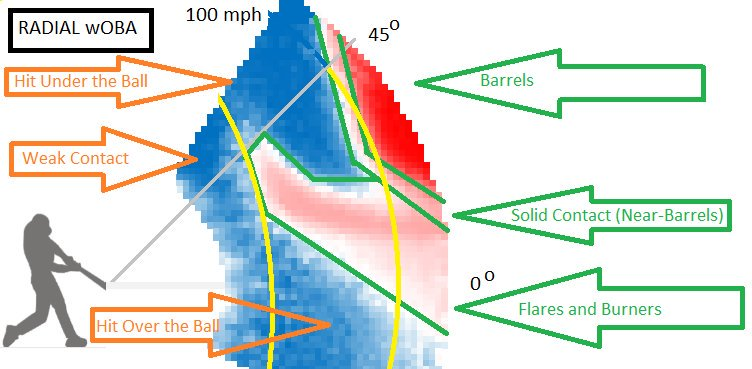
\includegraphics[width=\textwidth]{barrels.jpg}
\\
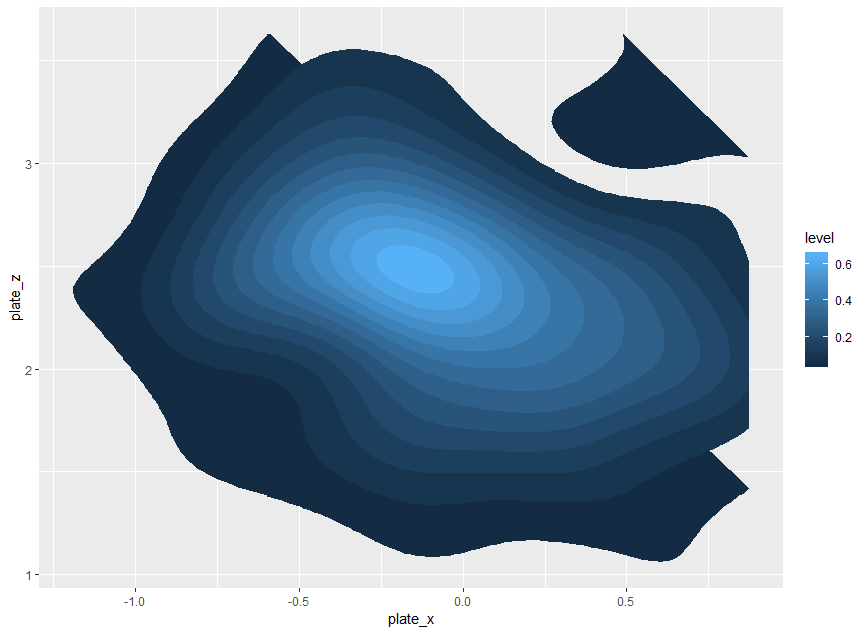
\includegraphics[width=\textwidth]{Rplot.png}

\pagebreak

\bibliographystyle{plain}
\bibliography{references}
\end{document}
